%!TEX root = informe.tex
\chapter{Análisis de Ciclo de Vida de un adoquín: definición del objetivo y alcance}\label{cap:acv_definicion}
\section{Objetivo}
Como se indicó en el capítulo \ref{cap:objeto}, el objetivo principal de este proyecto es el Análisis de Ciclo de Vida del adoquín común prefabricado del cemento utilizado en obras civiles y urbanismo, analizando el ciclo de vida del adoquín desde la obtención de la materia prima hasta su fin de vida, es decir, ``desde la cuna hasta la tumba''. El adoquín a estudio es el modelo Holanda 6, de dimensiones 200x100x60 \si{mm}.

La razón principal de este Análisis de Ciclo de Vida es evaluar el comportamiento ambiental de las distintas etapas de su ciclo de vida, las cargas ambientales asociadas a estas etapas e identificar las posibles mejoras.

El público al que se prevé comunicar los resultados de este estudio es principalmente al Tribunal Calificador de Proyectos y a los fabricantes de productos prefabricados del cemento.

No está previsto utilizar los resultados en aseveraciones comparativas con otros materiales y que puedan divulgarse al público.

\section{Alcance}
\subsection{Sistema y sus límites}
Según la norma UNE-EN-ISO 14044:2006 \cite{iso14044}, el \textbf{sistema del producto} ``representa el conjunto de procesos unitarios con sus flujos elementales y flujos de producto'', que para el caso de este proyecto se encuentra esquematizado en la figura \ref{fig:sistema}.

\begin{figure}[!htp]
\centering
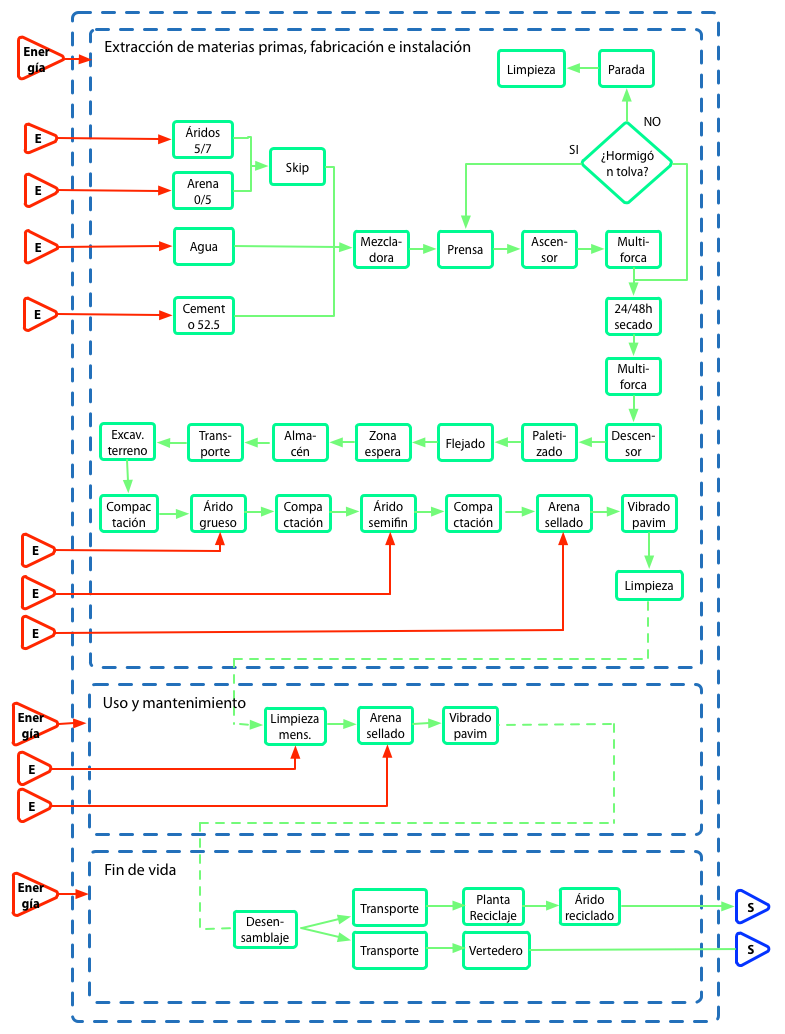
\includegraphics[height=18cm]{img/sistema.png}
\caption[Diagrama de flujo del sistema del producto adoquín.]{Diagrama de flujo del sistema del producto adoquín. Fuente: elaboración propia.}
\label{fig:sistema}
\end{figure}

También se define \textbf{proceso unitario} como ``el elemento más pequeño considerado en el análisis del inventario del ciclo de vida para el cual se cuantifican lo datos de entrada y salida'', siendo la \textbf{entrada} el ``flujo de producto, de materia o de energía que entra en un proceso unitario'' y la \textbf{salida} el ``flujo de producto, materia o de energía que sale de un proceso unitario''. Por último, el \textbf{flujo de producto} es ``productos que entran o salen de un sistema del producto hacia otro''. Sirva de ejemplo de proceso unitario en este caso el mezclado del hormigón o la vibrocompresión.

Para el estudio se ha empleado el modelo con mayor demanda de producción de la empresa Malaka de Prefabricados, S.L. y se han utilizado datos proporcionados de la misma (Anexo \ref{apend:datos}) para desarrollar el inventario y los cálculos. El adoquín a estudio es el modelo Holanda 6, de dimensiones 200x100x60 \si{mm} (datos técnicos en Anexo \ref{apend:catalogo}).

\subsection{Unidad funcional}\label{sec:unidad_funcional}
El motivo de tomar como \textit{Unidad funcional} ``1 \si{m^2} de adoquín'' es debido a que los pedidos y la fabricación se realizan en unidades de superficie y no en cantidad de bloques de adoquín. Cada bandeja fabricada supone exactamente 0.5 \si{m^2} de adoquines modelo ``Holanda 6''. Si se toma como \textit{Unidad funcional} 1 \si{m^2} de adoquín, los cálculos se realizan de forma sencilla para 2 bandejas.

\subsection{Límites del sistema}
Los \textbf{límites del sistema} ``definen los procesos unitarios a ser incluido en el sistema'', es decir ``determinan qué procesos unitarios se deben incluir dentro del ACV. La selección de los límites del sistema y la exclusión de etapas deben ser coherentes con los objetivos del estudio'' \cite{iso14040}:

\begin{itemize}
  \item No se ha excluido ninguna etapa en el análisis, aunque sea poco significativa.
  \item Los límites del sistema los establece el sistema del producto representado en la figura \ref{fig:sistema}. Las entradas/salidas no incluidas se consideran fuera del análisis.
  \item La cantidad total de adoquines son reciclables, aunque se indica que un 5\% se pierde en vertederos llegados allí mezclados con otros residuos \cite{euroadoquin}.
  \item Las capas componentes también pueden ser recicladas, pero sólo se tendrán en cuenta para la instalación y uso de los adoquines, ya que pueden reutilizarse para nuevas instalaciones tras un recambio de la capa de adoquines.
  \item Este proyecto se ha pensado para el área geográfica de Málaga en el año 2013 y tiene datos adaptados para tal caso. Es tal el caso del mix eléctrico, actualizado a fecha de 2013 para España \cite{mlgceballos}.
\end{itemize}

\subsection{Procedimientos de asignación}
Los procedimientos de asignación para futuras aseveraciones comparativas, en el caso que las haya, deberán incluir todas las entradas y salidas que se producen en cada proceso así como las consideradas en este proyecto. Se deberá evitar la omisión de etapas, procesos, entradas/salidas incluso en el caso de que no se altere de forma sustancial el resultado final.

\subsection{Categorías de impacto seleccionadas}\label{sec:categoriasimpactoseleccionadas}

Para la elección de las categorías de impacto, el método ReCiPe recoge 18 categorías, de las cuales se han seleccionado las más significativas según los objetivos y sistema elegidos:
\begin{itemize}
  \item Cambio climático — Salud humana (CC[HH]).
  \item Toxicidad humana (HT).
  \item Formación de partículas (PMF).
  \item Cambio climático - Ecosistemas (CC[Ec]).
  \item Ocupación de tierras agrícolas (ALO).
  \item Transformación natural de la tierra (NLT).
  \item Agotamiento de recursos fósiles (FD).
\end{itemize}

\subsection{Suposiciones}
La norma UNE-EN-ISO 14044:2006 \cite{iso14044} indica que ``se deben definir con claridad los criterios de corte para la inclusión inicial de entradas y salidas y las suposiciones sobre las cuales se establecen los criterios de corte'', las cuales son:

\begin{itemize}
  \item La distancia de recorrido desde la fuente de materias primas de áridos, arena y cemento es de 8 \si{km} (Alhaurín de la Torre) para las dos primeras y 30 \si{km} (Málaga-El Palo) para el cemento, ya que no siempre la materia prima procede del mismo sitio.
  \item Los cálculos de transporte se han realizado únicamente de ida para un camión de 16—32 \si{\tonne} que cumple una normativa europea de emisiones EURO 4.
  \item Las instalaciones donde se realiza el proceso de fabricación tienen una vida útil de 15 años.
  \item El uso del pavimento de adoquines al que se ha destinado es el arterias principales, que pertenece a la categoría de tráfico C1 y una calidad de explanada E2 con base granular.
  \item El sellado del pavimento de adoquines se hará únicamente con arena, evitando selladores cementados, para preservar la ventaja de fácil retirada para labores de mantenimiento o trabajo bajo explanada.
  \item La pérdida de arena entre periodos de mantenimiento del sellado del pavimento será del 50\% de la arena instalada inicialmente.
  \item El periodo de tiempo entre mantenimiento del sellado del pavimento será de 5 años, cumpliendo con las normas recomendadas \cite{euroadoquinc}.
  \item La distancia de recorrido desde el lugar de desensamblaje del adoquín hasta el vertedero o la planta de reciclado se ha supuesto de 50 \si{km} suponiendo una instalación en el área metropolitana de Málaga.
\end{itemize}

\subsection{Requisitos iniciales de calidad de los datos}
Como requisito de calidad de los datos se debe indicar que los datos han sido recopilados durante el año 2013, por lo que se deben considerar variaciones en los cálculos si se desea extrapolar a otros años. El área geográfica donde se han recopilado los datos es la provincia de Málaga (España).

Los datos de partida que se han utilizado en este análisis han sido proporcionados por Malaka de Prefabricados (Apéndice \ref{apend:datos}). La figura \ref{fig:sistema} muestra las entradas al sistema, así como los procesos que ocurren durante cada fase del ciclo de vida —que serán explicados en las siguientes secciones— y las salidas del sistema.
